% !TeX root = main.tex
% !TeX spellcheck = de_DE
% !TeX encoding = utf8
% !TeX root = main.tex
% !TeX spellcheck = de_DE
% !TeX encoding = utf8

\chapter{Error Correcting Codes}

For modern communications systems reliable data transmission and storage ist required. To achieve this goal usually error correcting codes are used. There are different possible codes available for error correction, but I will restrain myself to LDPC\cite{Ga63} codes in this thesis. As these codes can archive good performance and can be used at large block lengths\cite{TaSc2017}. This is especially useful for use with NAND based solid state drives.

When describing a block code there are important parameters as the message length $k$. The message is what is given into the encoder and the result from the decoder. The block length $n$, and the rate $R = k / n$. 

In this case error correction code are used to add additional information to data to allow errors. The errors are then corrected with that information. The addition of additional information is also called redundancy. With this redundancy it is possible to lose information while data is transmitted over a channel and decode it after the channel. After decoding the original data is recovered by using the additional information. \cref{channel_basic} shows such a system where information is transmitted, the channel can be of different type. It can for example be a wireless transmission or memory where information is first stored and later read back. 

\begin{figure}
	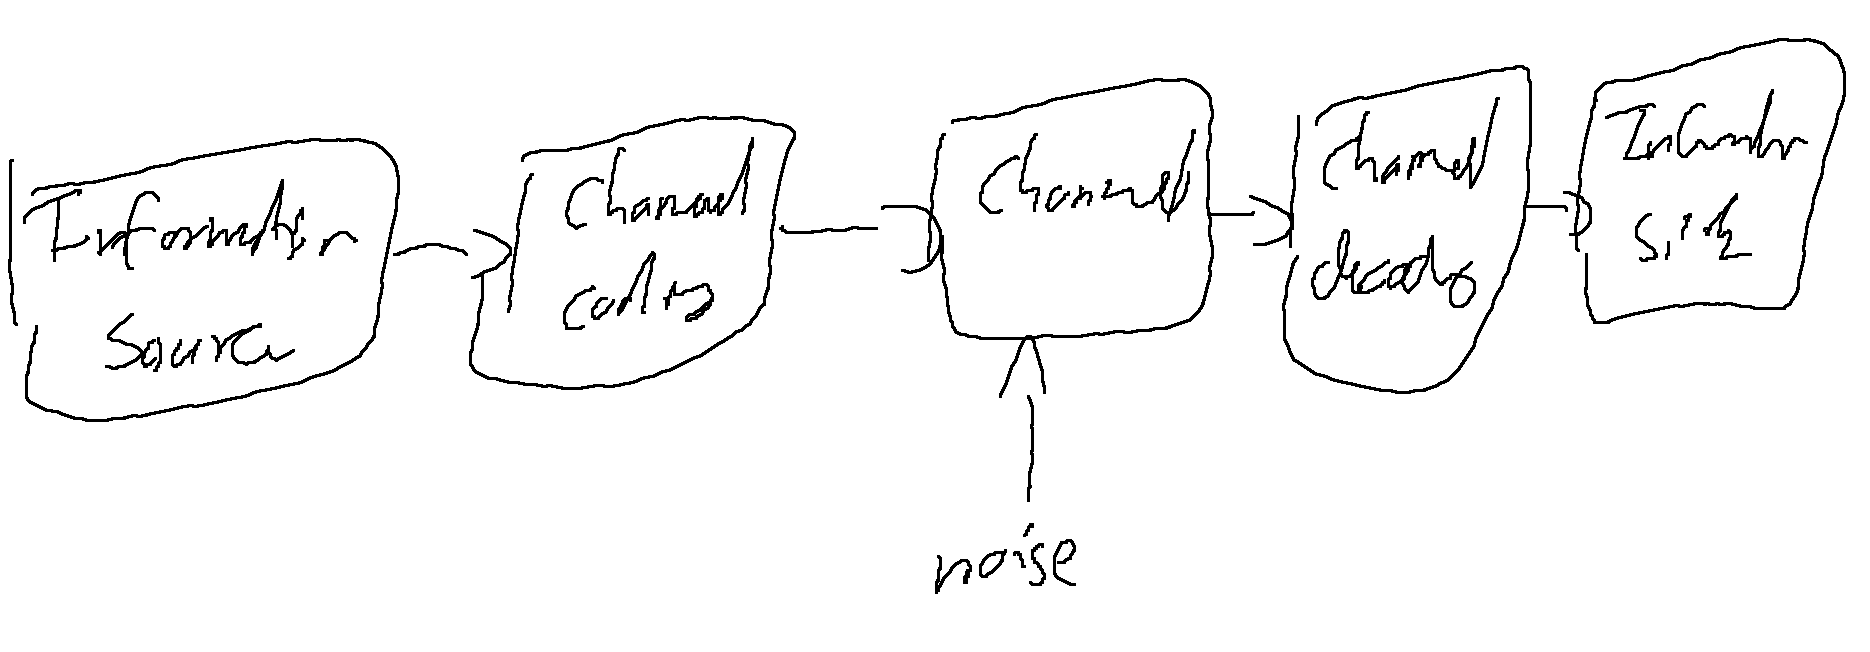
\includegraphics[width=10cm]{information_channel.png}
	
	\centering
	\caption{A basic channel where information is transmitted}	
	\label{channel_basic}
\end{figure}

\section{Low-Density Parity-Check (LDPC) Codes}

The following section will describe LDPC codes invented by Robert Gallager\cite{Ga63}. Starting with a graph representation I will describe the LDPC code and then continue with a matrix representation. LDPC codes can be shown as a bipartite graph also called Tanner graph\cite{Ta81} based on their inventor. \cref{tanner_ex} shows an example of one, where the check and parity nodes are connected by edges. This is an effective representation, moreover it will also help understanding the decoding algorithm later.

\begin{figure}
	\begin{tikzpicture}[
		cnode/.style={draw,rectangle,node distance=.5cm,align=center,minimum width=.5cm, minimum height=.5cm},
		vnode/.style={draw,circle,node distance=.5cm,align=center,minimum width=.5cm, minimum height=.5cm}
		]
		\node (vn) [vnode] {};
		\node [right=of vn] {code Symbols (variable nodes)};
		\node (cn) [below=of vn,cnode] {};
		\node [right=of cn] {parity equations (check nodes)};
	\end{tikzpicture}
	
	\begin{tikzpicture}[
		cnode/.style={draw,rectangle,node distance=1cm,align=center,minimum width=.5cm, minimum height=.5cm},
		vnode/.style={draw,circle,node distance=1cm,align=center,minimum width=.5cm, minimum height=.5cm}
	]
	\begin{scope}[start chain=going right, node distance=15mm]
		\node [vnode, on chain] (v0) {};
		\node [vnode, on chain] (v1) {};
		\node [vnode, on chain] (v2) {};
		\node [vnode, on chain] (v3) {};
		\node [vnode, on chain] (v4) {};
		\node [vnode, on chain] (v5) {};
		\node [vnode, on chain] (v6) {};
		\node [vnode, on chain] (v7) {};
	\end{scope}
	\begin{scope}[start chain=going right, node distance=15mm]
		\node [cnode, on chain, above=2cm of v2] (c0) {};
		\node [cnode, on chain] (c1) {};
		\node [cnode, on chain] (c2) {};
		\node [cnode, on chain] (c3) {};
	\end{scope}
	\draw (c0) -- (v1);
	\draw (c0) -- (v3);
	\draw (c0) -- (v4);	
	\draw (c0) -- (v7);
	\draw (c1) -- (v0);
	\draw (c1) -- (v1);
	\draw (c1) -- (v2);
	\draw (c1) -- (v5);
	\draw (c2) -- (v2);
	\draw (c2) -- (v5);
	\draw (c2) -- (v6);
	\draw (c2) -- (v7);
	\draw (c3) -- (v0);
	\draw (c3) -- (v3);
	\draw (c3) -- (v4);
	\draw (c3) -- (v6);
	\end{tikzpicture}
	\centering
	\caption{An example Tanner graph.}
	\label{tanner_ex}
\end{figure}

Instead of using the Tanner graph one can also use a matrix representation. In this matrix the ones represent the edges of the graph. Usually for a LDPC code the matrix is sparse or low density as the name implies. In \cref{ldpc_mat} a matrix representing the same code as in the graph in \cref{tanner_ex} is shown. The $\bm{H}$ matrix is of size $(n-k) \times n$. And the possible code words are given by the null space of $\bm{H}$, so in other words $c$ is a code word if and only if $c\bm{H}^T = \bm{0}$\cite{RiUr01}.


\begin{equation}
	\bm{H} = \left[\begin{matrix}
		0 & 1 & 0 & 1 & 1 & 0 & 0 & 1 \\ 
		1 & 1 & 1 & 0 & 0 & 1 & 0 & 0 \\
		0 & 0 & 1 & 0 & 0 & 1 & 1 & 1 \\
		1 & 0 & 0 & 1 & 1 & 0 & 1 & 0
	\end{matrix}\right] \label{ldpc_mat}
\end{equation}

\subsection{Quasicyclic LDPC (QC-LDPC) codes} \label{qc_ldpc}
LDPC codes can be difficult to implement, especially randomly generated ones. On the other hand structured codes can be devised to be more easily implemented. One class of these structured codes are quasicyclic LDPC codes. In these codes the parity check matrix is only built from circulant matrices and zero matrices\cite{Fo04}. The circulant matrices are defined by their first row as the following rows are the first one shifted. The base matrix specifies where zero matrices and where rotated circulant matrices are placed. Each circulant matrix has size $p\times$. The parity check matrix has size $(n-k) \times n = p (N - K) \times p N$. Thus the base matrix $\bm{B}$ has $(N - K) \times N$ entries. Often times the circulant matrix is the identity matrix and is rotated by the corresponding amount in the base matrix. In this base matrix the elements can be either a shift factor smaller that the circulant size $0 \leq b_{ij} < p$ or $-1$ representing a zero matrix.

In the following example the circulant matrix is a $5\times 5$ identity matrix. 
\begin{equation}
	\bm{B} = \left[\begin{matrix}
		-1 & 0 & 2 & -1\\
		0 & 1 & -1 & -1\\
		-1 & 1 & 0 & 2\\
	\end{matrix}\right]
\end{equation}
After the expansion the matrix looks like this:
\setcounter{MaxMatrixCols}{20}
\begin{equation}
	\bm{H} = \left[\begin{matrix}
		0 & 0 & 0 & 1 & 0 & 0 & 0 & 0 & 1 & 0 & 0 & 0 \\
		0 & 0 & 0 & 0 & 1 & 0 & 1 & 0 & 0 & 0 & 0 & 0 \\
		0 & 0 & 0 & 0 & 0 & 1 & 0 & 1 & 0 & 0 & 0 & 0 \\
		1 & 0 & 0 & 0 & 1 & 0 & 0 & 0 & 0 & 0 & 0 & 0 \\
		0 & 1 & 0 & 0 & 0 & 1 & 0 & 0 & 0 & 0 & 0 & 0 \\
		0 & 0 & 1 & 1 & 0 & 0 & 0 & 0 & 0 & 0 & 0 & 0 \\
		0 & 0 & 0 & 0 & 1 & 0 & 1 & 0 & 0 & 0 & 0 & 1 \\
		0 & 0 & 0 & 0 & 0 & 1 & 0 & 1 & 0 & 1 & 0 & 0 \\
		0 & 0 & 0 & 1 & 0 & 0 & 0 & 0 & 1 & 0 & 1 & 0 \\
	\end{matrix}\right]
\end{equation}
\todo{more qc specifics?}

\subsection{Encoding}
\subsubsection{Genrator Matrix}
For encoding the probably simplest algorithm is transforming the parity check matrix into systematic form $\bm{H} = \left[\begin{matrix} \bm{-A^T} & \bm{I_{n-k}}\end{matrix}\right]$. Where $\bm{I_{n-k}}$ is a $n-k \times n - k$ identity matrix and $\bm{A}$ has $k \times n - k$ elements. To archive this form one could for example use gaussian elimination. With $\bm{A}$ known we can construct the generator matrix $\bm{G} = \left[\begin{matrix} \bm{I_{k}} & \bm{A} \end{matrix}\right]$. Now encoding can be done with a simple matrix multiplication. With $u$ the information word and $v$ the code word is given by $v = \bm{G}u$.

Take for example the matrix from \cref{ldpc_mat}. If we use gaussian elimination to bring the right side to identity we are left with \cref{ldpc_ident}. Now we take the left part of the matrix and transpose it to get $\bm{A}$. With we build $\bm{G}$ in \cref{ldpc_gen}.

\begin{align}
	\bm{H} = \left[\begin{matrix}
		0 & 1 & 0 & 1 & 1 & 0 & 0 & 0 \\
		1 & 1 & 1 & 0 & 0 & 1 & 0 & 0 \\
		1 & 1 & 0 & 0 & 0 & 0 & 1 & 0 \\
		0 & 0 & 0 & 0 & 0 & 0 & 0 & 1
	\end{matrix} \right] \label{ldpc_ident} \\
	\bm{G} = \left[\begin{matrix}
		0 & 1 & 1 & 0 & 1 & 0 & 0 & 0 \\
 		1 & 1 & 1 & 0 & 0 & 1 & 0 & 0 \\
 		0 & 1 & 0 & 0 & 0 & 0 & 1 & 0 \\
 		1 & 0 & 0 & 0 & 0 & 0 & 0 & 1
	\end{matrix} \right] \label{ldpc_gen}
\end{align}

The main disadvantage of this strategy is the high computational complexity. When transforming the parity check matrix into systematic form we have a complexity of $\mathcal{O}(n^3)$. This is not to bad as it will mostly be done offline and only the $\bm{G}$ matrix stored in the encoder, but the bigger problem is that due to the gaussian elimination the matrix is no longer sparse. Thus the matrix multiplication will result in a complexity of $\mathcal{O}(n^2)$\cite{QiGo07}. 

\subsubsection{Approximate Lower Triangular Form} \label{alt_enc_alg}
Richardson and Urbanke\cite{RiUr01} describe a way to reorder the parity check matrix to reduce the encoding complexity. They bring the matrix into a so called approximate lower triangular form. This is done by only doing row and column permutation, so the low density of the matrix is kept. The resulting structure of the matrix is shown in \cref{alt_mat}. Especially advantageous is the reduced complexity for encoding, here the encoding complexity is reduced from $\mathcal{O}(n^2)$ to $\mathcal{O}(n + g^2)$, where $g$ is the gap. This gap is the number of rows that cannot be brought into triangular form, as seen in \cref{alt_mat}. We can also write
\begin{figure}
	\begin{tikzpicture}[
		style1/.style={
				matrix of math nodes,
				every node/.append style={text width=#1,align=center,minimum height=3ex},
				nodes in empty cells,
			}
		]
		\matrix[style1=0.3cm] (1mat) {
			& & & & & & & & & & & & & & & \\
			& & & & & & & & & & & & & & & \\
			& & & & & & & & & & & & & & & \\
			& & & & & & & & & & & & & & & \\
			& & & & & & & & & & & & & & & \\
			& & & & & & & & & & & & & & & \\
			& & & & & & & & & & & & & & & \\
			& & & & & & & & & & & & & & & \\
		};
		\draw[dashed] (1mat-5-1.south west) -- (1mat-5-16.south east);
		\draw[dashed] (1mat-1-11.north east) -- (1mat-8-11.south east);
		\draw[dashed] (1mat-1-8.north east) -- (1mat-8-8.south east);

		\node [font=\Large] at ($(1mat-3-4)!0.5!(1mat-3-5)$) {$\bm{A}$};
		\node [font=\Large] at (1mat-3-10) {$\bm{B}$};

		\node [font=\Large] at (1mat-4-13) {$\bm{T}$};
		\node [font=\Large] at (1mat-2-15) {$\bm{0}$};

		\node [font=\Large] at ($(1mat-7-4)!0.5!(1mat-7-5)$) {$\bm{C}$};
		\node [font=\Large] at (1mat-7-10) {$\bm{D}$};
		\node [font=\Large] at (1mat-7-14) {$\bm{E}$};

		\node at (1mat-1-12) {1};
		\node at (1mat-2-13) {1};
		\node at (1mat-3-14) {1};
		\node at (1mat-4-15) {1};
		\node at (1mat-5-16) {1};
		
		\draw (1mat-1-1.north west) -- (1mat-8-1.south west);
		\draw (1mat-1-16.north east) -- (1mat-8-16.south east);
		\draw (1mat-1-1.north west) -- (1mat-1-16.north east);
		\draw (1mat-8-1.south west) -- (1mat-8-16.south east);

		\draw [<->] ([yshift=-3mm]1mat-8-1.south west) -- node[below] {$n$} ([yshift=-3mm]1mat-8-16.south east);
		\draw [<->] ([xshift=-3mm]1mat-1-1.north west) -- node[left] {$m$} ([xshift=-3mm]1mat-8-1.south west);

		\draw [<->] ([yshift=3mm]1mat-1-1.north west) -- node[above] {$n-m$} ([yshift=3mm]1mat-1-8.north east);
		\draw [<->] ([yshift=3mm]1mat-1-9.north west) -- node[above] {$g$} ([yshift=3mm]1mat-1-11.north east);
		\draw [<->] ([yshift=3mm]1mat-1-12.north west) -- node[above] {$m-g$} ([yshift=3mm]1mat-1-16.north east);

		\draw [<->] ([xshift=3mm]1mat-1-16.north east) -- node[right] {$m-g$} ([xshift=3mm]1mat-5-16.south east);
		\draw [<->] ([xshift=3mm]1mat-6-16.north east) -- node[right] {$g$} ([xshift=3mm]1mat-8-16.south east);


	\end{tikzpicture}
	\centering
	\caption{Structure of a matrix in approximate lower triangular form.}
	\label{alt_mat}
\end{figure}
\begin{equation}
	\bm{H} = \left[\begin{matrix}
		\bm{A} & \bm{B} & \bm{T} \\
		\bm{C} & \bm{D} & \bm{E}
	\end{matrix} \right]
	\label{alt_subs}
\end{equation}
the submatrices all have the dimensions given in \cref{alt_mat}. By multiplying \cref{alt_subs} with
\begin{equation}
	\left[\begin{matrix}
		\bm{I} & \bm{0} \\
		-\bm{E}\bm{T}^{-1} & \bm{I}
	\end{matrix} \right]
\end{equation}
the resulting matrix is
\begin{equation}
	\left[\begin{matrix}
		\bm{A} & \bm{B} & \bm{T} \\
		-\bm{E}\bm{T}^{-1}\bm{A} + \bm{C} & -\bm{E}\bm{T}^{-1}\bm{B} + \bm{D} & \bm{0}
	\end{matrix}\right]
\end{equation}
. By splitting the codeword into three parts $c = \left[\begin{matrix}s & p_1 & p_2\end{matrix}\right]$ and applying the definition for valid code words $\bm{H}^T = \bm{0}$. It splits into
\begin{align}
	\bm{A}s^T + \bm{B}p_1^T + \bm{T}p_2^T & = 0	\\
	\left(-\bm{E}\bm{T}^{-1}\bm{A} + \bm{C}\right)s^T + \left(-\bm{E}\bm{T}^{-1}\bm{B} + \bm{D}\right)p^T & = 0
\end{align}
. The resulting equations for $p_1$ and $p_2$ are
\begin{align}
	p_1^T & = -\bm{\phi}^{-1}\left(-\bm{E}\bm{T}^{-1}\bm{A} + \bm{C}\right)s^T \label{p1_calc}\\
	p_2^T & = -\bm{T}^{-1}\left(\bm{A}s^T + \bm{B}p_1^T\right) \label{p2_calc}
\end{align}
. The complexity of the computations can be reduced by computing $\bm{\phi}^{-1}$ offline. Offline meaning that it is precomputed and when encoding multiplying by the matrix. All the other matrix multiplications from \cref{p1_calc,p2_calc} are done separately. Multiplications by $\bm{A}$, $\bm{B}$, $\bm{C}$, and $\bm{E}$ are sparse and the resulting complexity for these is $\mathcal{O}(n)$. The multiplication with $\bm{T}^{-1}$ is replaced by the system $x^T = \bm{T}y^T$. As $\bm{T}$ is a sparse lower triangular matrix the system can be solved by back substitution in $\mathcal{O}(n)$. The only part with higher complexity is the multiplication with the dense $g\times g$ matrix $\bm{\phi}$ where the complexity is $\mathcal{O}(g^2)$. 

\begin{table}
	\begin{tabular}{l l}
		Operation & Type \\ \toprule
		$\bm{A}s^T$ & sparse multiplication \\
		$\bm{T}^{-1}\bm{A}s^T$ & sparse back substitution \\
		$-\bm{E}\bm{T}^{-1}\bm{A}s^T$ & sparse multiplication \\
		$\bm{C}s^T$ & sparse multiplication \\
		$\left(-\bm{E}\bm{T}^{-1}\bm{A}s^T\right) + \left(\bm{C}s^T\right)$ & vector addition \\
		$\bm{\phi}^{-1}\left(-\bm{E}\bm{T}^{-1}\bm{A}s^T + \bm{C}s^T\right)$ & dense $g\times g$ multiplication\\
	\end{tabular}
	\centering
	\caption{Calculations for $p_1^T = \bm{\phi}^{-1}\left(-\bm{E}\bm{T}^{-1}\bm{A} + \bm{C}\right)s^T$}
	\label{p1_steps}
\end{table}
\begin{table}
	\begin{tabular}{l l}
		Operation & Type \\ \toprule
		$\bm{A}s^T$ & sparse multiplication \\
		$\bm{B}p_1^T$ & sparse multiplication \\
		$\left(\bm{A}s^T\right) + \left(\bm{B}p_1^T\right)$ & vector addition \\
		$-\bm{T}^{-1}\left(\bm{A}s^T + \bm{B}p_1^T\right)$ & sparse back substitution \\
	\end{tabular}
	\centering
	\caption{Calculations for $p_2^T = -\bm{T}^{-1}\left(\bm{A}s^T + \bm{B}p_1^T\right)$}
	\label{p2_steps}
\end{table}
\todo{do i want do describe the algorithm to get into alt form? yes!}

\subsection{Decoding}
Decoding LDPC codes is a nontrivial problem, in fact maximum likelihood decoding is computationally infeasible. Therefore other decoding methods were developed. There are different decoding algorithms which differ in performance and complexity. I will start with a simple algorithm to introduce the required concepts and then go on to more performant ones.

\subsubsection{Hard Descision Decoding}
This algorithm works on binary input data and all the messages are also binary. The decoder basically follows the Tanner graph. All messages are passed along the edges and computations are made on the nodes. 



\todo{decode dat }

